\documentclass[11pt]{article}

% Packages
\usepackage{amsmath}
\usepackage{enumitem}
\usepackage{graphicx}
    \graphicspath{ {../images/labs} }
% Document
\begin{document}
    \begin{enumerate}
        \item A stomach cell line growing in nutrient broth has a mutation in the gene encoding a particular
type of tRNA. Assuming the mutation is not lethal to the cells, explain why the amount
of SIRT3 mRNA in this cell line is identical to the amount produced by a normal stomach (NSNS)
cell line but the amount of SIRT3 protein is less than in the NS cells.
        \begin{enumerate}
            \item There could be a few answers, but the most likely is that the gene is not being expressed.
            This is backed up from \ref{Figure 1}
        \end{enumerate}
    \end{enumerate}

\newpage
    Figures.

    \begin{figure}
        \caption{Figure 1}
        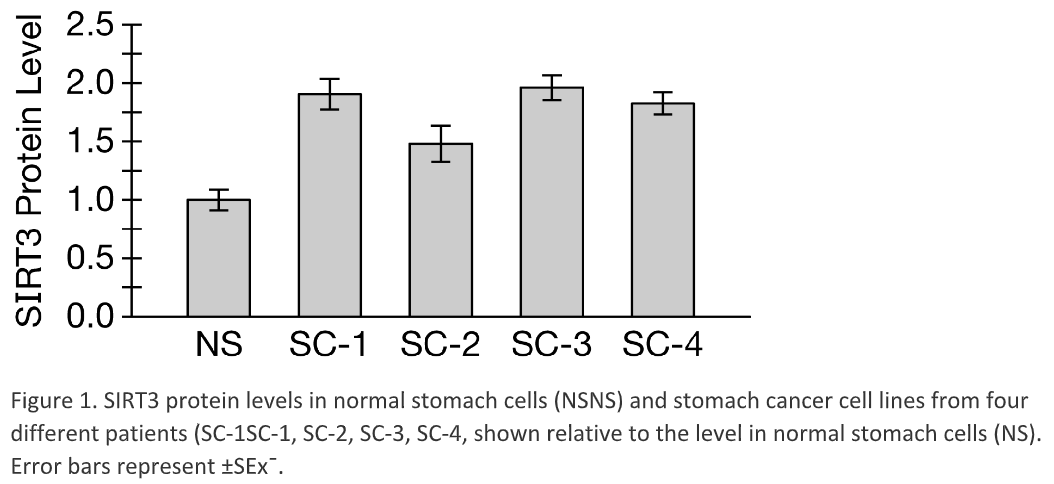
\includegraphics{Long FRQ Fig. 1}
        \label{Figure 1}
    \end{figure}






\end{document}